\subsection{Anlage A - Zeitplanung}
\label{anlage:zeitplanung}

\begin{figure}[h]
    \centering
    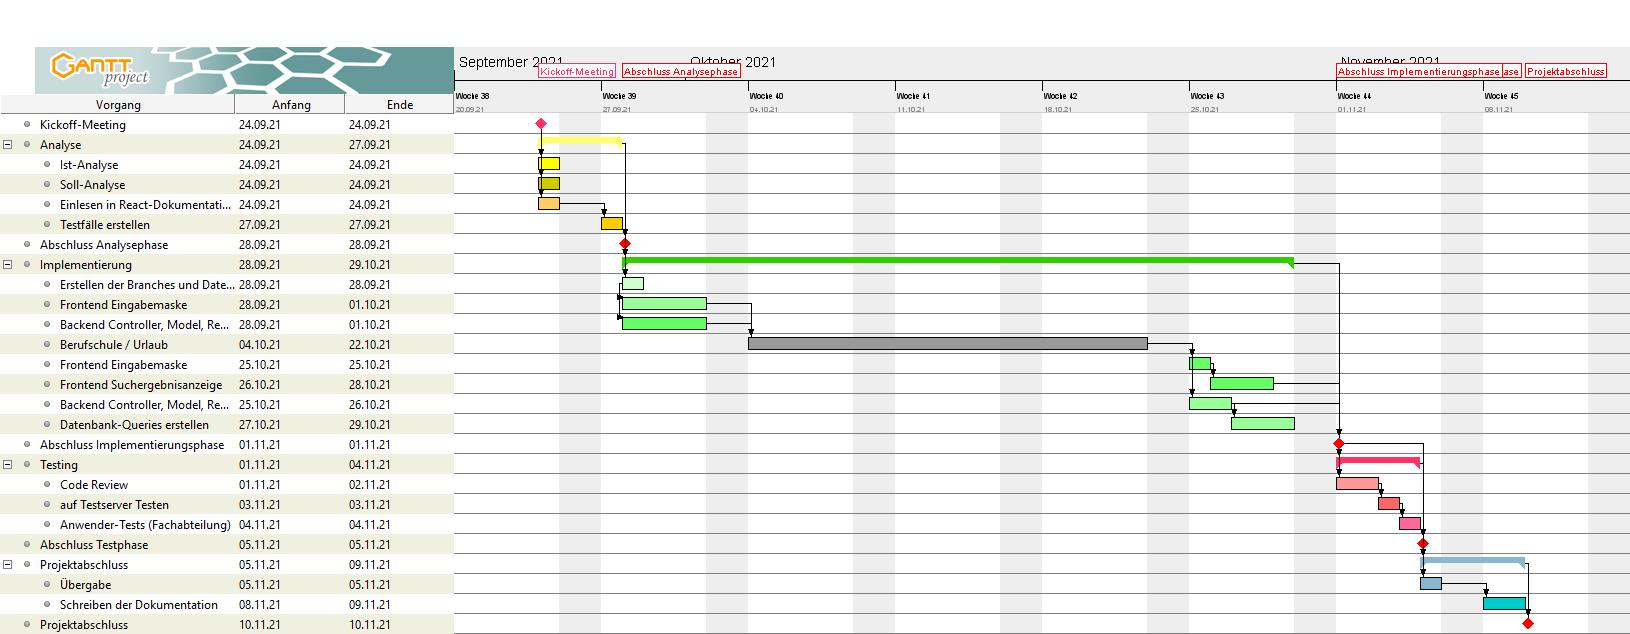
\includegraphics[angle=90, origin=c,width=0.45\textwidth]{zeitplanung.jpg}
    \caption{Gantt-Diagramm zur Projektzeitplanung}
\end{figure}

\pagebreak
\subsection{Anlage B - Ressourcenplanung}
\label{anlage:ressourcen}

{\textbf{Hardware}}
    \begin{itemize}
        \item Büroarbeitsplatz
        \item 2 Monitore
        \item 1 Dockingstation
        \item 1 Laptop
        \item Maus, Tastatur
    \end{itemize}

{\textbf{Software}}
    \begin{itemize}
        \item Virtuelle Maschine mit Fedora 32 mit folgender Software:
        \begin{itemize}
            \item Docker-basierte Entwicklungsumgebung
            \item MySQL Datenbank \& -server
            \item Proxyserver (Squid)
            \item Quelltext-Repositories des Backend Relaunches
        \end{itemize}
        \item Notebook mit Windows 10 Enterprise mit folgender Software
        \begin{itemize}
            \item PHPStorm
            \item Visual Studio Code
            \item SQLyog Ultimate 64 (Datenbankmanagementsystem)
            \item Google Chrome
            \item Mozilla Firefox
            \item Git
            \item Jira - Projektmanagementsystem (Webanwendung)
        \end{itemize}
    \end{itemize}

{\textbf{Personal}}
    \begin{itemize}
        \item Auszubildender, Entwickler - Projektumsetzung
        \item Fachbetreuer, Entwickler - Beratung, Code Review
        \item Mitarbeiter Abteilung IT - Code Review
        \item Mitarbeiter Fachabteilung Human Resources - Tests, Projektabnahme
    \end{itemize}
\pagebreak

\subsection{Anlage C - Kostenanalyse}
\label{anlage:kosten}

\begin{table}[h]
    \centering
    \begin{tabular}{p{3cm} ccc p{3cm} p{3cm} p{3cm}}
        & Auszubildender & Mitarbeiter HR & Mitarbeiter IT\\
        \hline
        monatliches \mbox{Gehalt} & 1.350 € & 1.900 € & 2.500 € \\
        Arbeitstage\,/ \mbox{Monat} & 21 & 21 & 21\\
        Stunden\,/ Tag & 8 & 8 & 8\\
        effektiver \mbox{Stundensatz} & 8,04 € & 11,31 € & 14,88 €\\
        Betriebskosten\,/ Tag & 20 € & 20€ & 20 €\\
        Mannstunden & 120 & 4 & 6\\
        Kosten & 1.264,29 € & 55,24 € & 104,29 €\\
        \hline
        Gesamtkosten & & & \underline{\underline{1.423,81 €}}
    \end{tabular}
\end{table}
\pagebreak

\subsection{Anlage D - ERD}
\label{anlage:erd}

\begin{figure}[h]
    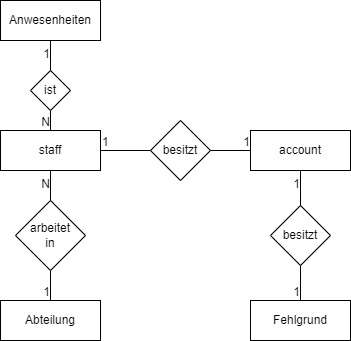
\includegraphics[width=\textwidth]{ERD.jpg}
    \caption{Entity-Relationship-Diagramm der Mitarbeiter-Tabellen}
\end{figure}
\pagebreak

\subsection{Anlage E - Testprotokoll}
\label{anlage:test}

\begin{table}[h]
    \centering
    %\begin{tabular} { |p{0.5cm}|p{7.5cm}|p{2cm}|p{2cm}|}
    \begin{tabular}{|m{0.5cm}|m{9cm}|m{2.5cm}|m{2cm}|}
        \hline
        Nr. & Testfall & Ergebnis & Status\\
        \hline
        1 & Tool in Admin Dropdown auswählen & Tool wird geladen & Erfolgreich\\ \hline
        2 & Eingabe in Inputfelder & Eingabe wird übernommen & Erfolgreich\\ \hline
        3 & Eingabe unerlaubter Zeichen & Zeichen wird nicht in Input übernommen & Erfolgreich\\ \hline
        4 & Suche ohne Vor-, Nachname oder Abteilung & Ausgabe aller Mitarbeiter & erfolgreich\\ \hline
        5 & Suche mit unvollständigem Vornamen & Ausgabe aller passenden Mitarbeiter & Erfolgreich\\ \hline
        6 & Suche mit unvollständigem Nachnamen & Ausgabe aller passenden Mitarbeiter & Erfolgreich\\ \hline
        7 & Suche nur mit ausgewählter Abteilung & Anzeige aller Mitarbeiter in Abteilung & Erfolgreich\\ \hline
        8 & Suche mit vollständigem Namen & Zutreffender Mitarbeiter wird angezeigt & Erfolgreich\\ \hline
        9 & Klick auf Nachnamen in Suchergebnissen & Weiterleitung in Profilansicht & Erfolgreich\\ \hline
        10 & Klick auf \glqq Back\grqq{} Button & Zurück zur Suchansicht & Erfolgreich\\ \hline
        11 & Aufruf der Profilansicht über URL \mbox{(backend.unitedprint.dev/other/contacts/1234)} & Weiterleitung in Profilansicht & Erfolgreich\\ \hline
    \end{tabular}
\end{table}
\pagebreak

\subsection{Anlage F - Softwareschnittstellen}
\textbf{API Routen}
\begin{itemize}
    \item Get-Request Routen
    \begin{itemize}
        \item /employee/{id}
        \begin{itemize}
            \item Übergabeparameter: Mitarbeiter-ID (über URL)
            \item Rückgabewert: Datensatz mit detaillierten Daten zum Mitarbiter in Form:\\
            {[id, name, vorname, abteilung, ... ]}
        \end{itemize}
        \item /get-branches
        \begin{itemize}
            \item Übergabeparameter: nichts
            \item Rückgabewert: Multidimensionales Objekt mit hierearchisch geordneten Abteilungen in Form:\\
            \{[id], [id, child = [id]],[id] \}
        \end{itemize}
    \end{itemize}

    \item Post-Request Routen
    \begin{itemize}
        \item /employee
        \begin{itemize}
            \item Übergabeparameter: JSON-Objekt mit Vor-, Nachnamen und / oder Abteilungs-ID
            \item Rückgabewert: Array mit zutreffenden Datensätzen in Form:\\
            \{ {[}mitarbeiter1{]}, {[}mitarbeiter2{]}, ... \}

        \end{itemize}
    \end{itemize}
\end{itemize}
\pagebreak

\subsection{Anlage G - Listing PHP Funktion \glqq groupBranches\grqq{}}
\vspace{1cm}
\begin{lstlisting}[language=PHP, numbers=left, tabsize=2]
    private function groupBranches(Collection $branchesCollection,
                                    int $id = 0): array
    {
    $branchesHierarchic  [];

    foreach ($branchesCollection as $branch) {
      if ($branch->group === $id) {
          $branchesHierarchic[] = [
              "id"     => $branch->id,
              "group"  => $branch->group,
              "branch" => $branch->branch,
              "rank"   => $branch->rank
          ];

          $children = $this->groupBranches(
              $branchesCollection,
              $branch->id
          );

          if (!empty($children)) {
              $branchesHierarchic[sizeof($branchesHierarchic) - 1]
                  ['children'] = $children;
          }
      }
    }

    }
\end{lstlisting}